\documentclass[11pt,a4paper]{article}

\usepackage[T1]{fontenc}
\usepackage[utf8]{inputenc}
\usepackage{lmodern}
\usepackage[margin=22mm,headheight=15pt]{geometry}
\usepackage{graphicx}
\usepackage{booktabs}
\usepackage{tabularx}
\usepackage{longtable}
\usepackage{array}
\usepackage{multirow}
\usepackage{enumitem}
\usepackage{siunitx}
\usepackage{xcolor}
\usepackage{tikz}
\usetikzlibrary{arrows.meta,positioning,fit,backgrounds,shapes.geometric,calc}
\usepackage{listings}
\usepackage{float}
\usepackage[section]{placeins}
\usepackage{caption}
\usepackage{subcaption}
\usepackage{fancyhdr}
\usepackage{lastpage}
\usepackage{titlesec}
\usepackage{hyperref}

\definecolor{navy}{HTML}{12314A}
\definecolor{teal}{HTML}{138A8A}
\definecolor{sky}{HTML}{DDEFF4}
\definecolor{pale}{HTML}{F3F7F8}
\definecolor{amber}{HTML}{D88A16}
\definecolor{redx}{HTML}{B33A3A}
\definecolor{greenx}{HTML}{2F7D4A}
\definecolor{greyx}{HTML}{58656E}

\hypersetup{
  colorlinks=true,
  linkcolor=navy,
  citecolor=teal,
  urlcolor=teal,
  pdftitle={CubeSat: A Brief Overview},
  pdfauthor={MD AHADUL HAQUE SUVO}
}

\pagestyle{fancy}
\fancyhf{}
\lhead{CubeSat: A Brief Overview}
\rhead{Technical Report}
\cfoot{\thepage\ of \pageref{LastPage}}
\renewcommand{\headrulewidth}{0.4pt}

\titleformat{\section}{\Large\bfseries\color{navy}}{\thesection}{0.7em}{}
\titleformat{\subsection}{\large\bfseries\color{navy}}{\thesubsection}{0.7em}{}
\titleformat{\subsubsection}{\normalsize\bfseries\color{teal}}{\thesubsubsection}{0.7em}{}

\setlist[itemize]{leftmargin=1.5em,itemsep=2pt,topsep=3pt}
\setlist[enumerate]{leftmargin=1.7em,itemsep=2pt,topsep=3pt}
\setlength{\parindent}{0pt}
\setlength{\parskip}{5pt}
\raggedbottom

\newcommand{\code}[1]{\texttt{#1}}
\newcommand{\src}[2]{\texttt{\footnotesize #1:}\allowbreak\texttt{\footnotesize #2}}
\newcommand{\status}[2]{\textcolor{#1}{\textbf{#2}}}
\newcommand{\repo}{\href{https://github.com/SISIYAM/sensorTest}{SISIYAM/sensorTest}}
\newcommand{\critical}{\status{redx}{Critical}}
\newcommand{\high}{\status{amber}{High}}
\newcommand{\medium}{\status{teal}{Medium}}
\newcommand{\low}{\status{greyx}{Low}}

\newcolumntype{Y}{>{\raggedright\arraybackslash}X}
\newcolumntype{P}[1]{>{\raggedright\arraybackslash}p{#1}}

\lstdefinestyle{embedded}{
  language=C++,
  basicstyle=\ttfamily\footnotesize,
  keywordstyle=\color{navy}\bfseries,
  commentstyle=\color{greyx}\itshape,
  stringstyle=\color{teal},
  numbers=left,
  numberstyle=\tiny\color{greyx},
  frame=single,
  rulecolor=\color{sky},
  backgroundcolor=\color{pale},
  breaklines=true,
  showstringspaces=false,
  xleftmargin=1.6em,
  framexleftmargin=1.2em
}

\begin{document}

\begin{titlepage}
\thispagestyle{empty}
\color{black}
\begin{center}
\vspace*{16mm}
{\Large\bfseries AVIATION AND AEROSPACE UNIVERSITY\par}
\vspace{5mm}
{\large SOFTWARE AND SIGNAL PROCESSING TEAM\par}

\vspace{18mm}
\rule{0.78\textwidth}{0.7pt}\par

\vspace{35mm}
{\Huge\bfseries CubeSat\par}
\vspace{7mm}
{\LARGE A Brief Overview\par}

\vspace{15mm}
{\large\bfseries TECHNICAL REPORT\par}
\vspace{6mm}
{\normalsize Hardware, Firmware, Sensor Integration, Imaging,\par
Navigation, Storage, and Engineering Readiness Assessment\par}

\vfill
\rule{0.55\textwidth}{0.5pt}\par
\vspace{9mm}
\begin{tabular}{@{}rl@{}}
\textbf{Prepared by:} & MD AHADUL HAQUE SUVO\\[2mm]
\textbf{Prepared for:} & Software and Signal Processing Team\\[2mm]
\textbf{Institution:} & Aviation and Aerospace University\\[2mm]
\textbf{Report date:} & 18 August 2026
\end{tabular}
\vspace{20mm}
\end{center}
\end{titlepage}

\pagenumbering{roman}
\tableofcontents
\clearpage
\pagenumbering{arabic}

\section{Executive assessment}

The reviewed repository implements a compact, proof-of-concept sensor and imaging hub around an ATmega2560-class controller. The code integrates an I\textsuperscript{2}C inertial/environmental cluster, an SPI BME680, three analogue channels, a UART GPS receiver, an ArduCAM OV2640 camera, and SD-card image storage. Its strongest design decision is explicit chip-select arbitration for three peripherals sharing the Mega hardware-SPI bus. A 256-byte transfer buffer also respects the ATmega2560's limited SRAM while the camera module retains a complete frame in its external FIFO.

The present revision is suitable as a laboratory integration baseline, but it is not yet a dependable payload controller and must not be represented as flight-ready. Four issues dominate that conclusion. First, the L3G4200D is detected but never placed into measurement mode; the subsequent byte assembly also omits signed conversion and sensitivity scaling. Second, image capture can block indefinitely, while filename reuse after reset can append a new JPEG to an existing file. Third, the software has no persistent sensor-health state, timestamped telemetry record, watchdog recovery, or build/dependency lock. Fourth, the repository contains no PCB manufacturing evidence, power tree, level-shifting scheme, or qualification record. The NEO-6M's documented operational envelope is also incompatible with orbital CubeSat navigation, although it remains useful for terrestrial bench tests.

\begin{table}[H]
\centering
\caption{Decision-oriented status summary at revision \code{28d356c}.}
\label{tab:summary}
\begin{tabularx}{\textwidth}{P{0.24\textwidth}P{0.19\textwidth}Y}
\toprule
Assessment area & Status & Engineering interpretation\\
\midrule
Repository scope & \status{teal}{Firmware prototype} & Four tracked files and five commits; no PCB or test artefacts are versioned.\\
Bus architecture & \status{greenx}{Coherent with caveats} & I\textsuperscript{2}C, SPI, UART, and ADC allocation is conceptually viable; SPI ownership and voltage domains require physical verification.\\
Sensor acquisition & \status{amber}{Partially valid} & Library-based sensors expose engineering units, but the gyroscope and analogue sensors are not measurement-ready.\\
Imaging and storage & \status{amber}{Functional concept} & Event-driven JPEG capture and chunked SD writing are implemented; timeout, file integrity, and reset-safe naming are missing.\\
Fault tolerance & \status{redx}{Insufficient} & Fatal SD halt, unchecked I\textsuperscript{2}C reads, no watchdog, no degraded mode, and no persistent health bitmap.\\
CubeSat readiness & \status{redx}{Not demonstrated} & Electrical, thermal-vacuum, radiation, vibration, EMC, and mission-level verification evidence is absent.\\
\bottomrule
\end{tabularx}
\end{table}

The most efficient next step is not a wholesale redesign. It is a controlled maturation sequence: freeze a reproducible build, correct the deterministic firmware defects, establish a timestamped binary/CSV telemetry contract, verify each voltage and interface on the physical board, and then perform integrated fault-injection and environmental tests. Section~\ref{sec:roadmap} provides acceptance criteria for that progression.

\section{Scope, evidence, and method}

\subsection{Repository baseline}

Repository identity, revision history, and file inventory were verified directly against the public project \cite{repo}.

The source of truth is the public GitHub repository \repo, default branch \code{main}, at commit \code{28d356c}. The repository was created in December 2025 and contains five commits through January 2026. The current tree consists of a wiring-oriented README and three firmware files. The three source files contain 556 physical lines in total. No release tag, licence, continuous-integration workflow, dependency manifest, schematic, PCB source, Gerber, bill of materials, test log, or sample dataset is present.

\begin{table}[H]
\centering
\caption{Version-controlled evidence reviewed in this assessment.}
\label{tab:repo}
\begin{tabularx}{\textwidth}{P{0.25\textwidth}P{0.14\textwidth}P{0.14\textwidth}Y}
\toprule
Artefact & Physical lines & Role & Audit significance\\
\midrule
\code{main/main.ino} & 239 & Application orchestration & Initialisation, cooperative schedule, serial telemetry, camera capture, and SD transfer.\\
\code{main/SensorHub.h} & 68 & Public sensor abstraction & Declares sensor objects, pins, measurements, and GPS state.\\
\code{main/SensorHub.cpp} & 249 & Driver composition & Probes and reads sensors, configures BME680, parses GPS, and controls the gas-sensor preheat pin.\\
\code{readme.md} & 145 & Wiring notes & Documents intended modules and pin connections, but contains two material inconsistencies with the code.\\
\bottomrule
\end{tabularx}
\end{table}

\subsection{Assessment boundaries}

The analysis combines static code inspection, commit-history inspection, interface tracing, timing analysis, and comparison against manufacturer or project-owner documentation. A statement is treated as \emph{implemented} only when supported by executable code, \emph{documented} when it appears only in the README, and \emph{unverified} when it depends on a physical design or test record that is absent.

This distinction is essential. A pin table does not establish voltage compatibility; a successful \code{begin()} call does not establish calibrated accuracy; and consumer component specifications do not establish performance in vacuum, radiation, launch vibration, or the mission thermal cycle. No hardware was available for electrical probing, and the local environment did not contain an Arduino build toolchain. Therefore, the report does not claim a reproduced build or measured sensor performance.

\section{System architecture}

\subsection{Functional partitioning}

Figure~\ref{fig:architecture} reconstructs the system from the code and README. The ATmega2560 is the single control and scheduling authority. Four interface domains converge at the controller: a shared I\textsuperscript{2}C bus for the GY-801 devices and camera configuration, a shared SPI bus for BME680, camera FIFO, and SD storage, one hardware UART for NMEA navigation data, and three ADC channels for gas and ultraviolet front ends. USB serial is used as the command and human-readable telemetry channel.

\begin{figure}[H]
\centering
\resizebox{0.97\textwidth}{!}{%
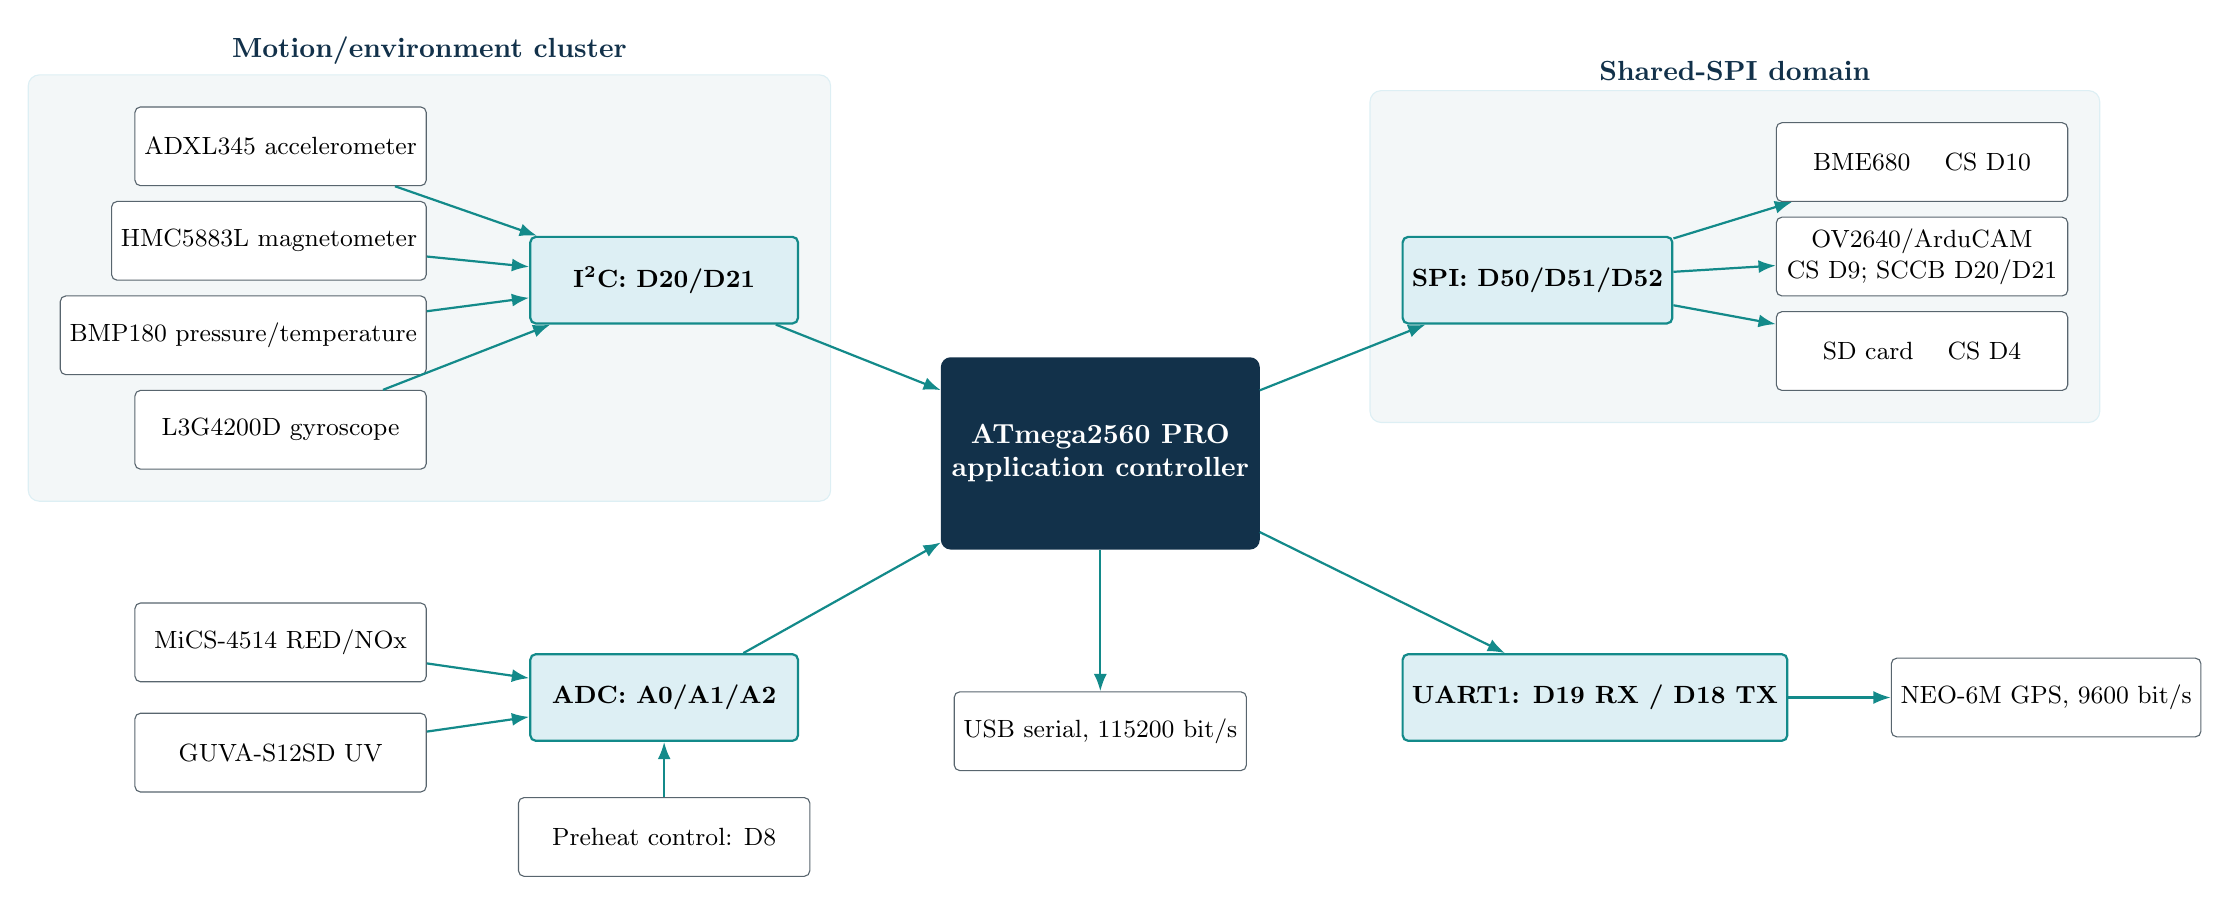
\begin{tikzpicture}[
  node distance=9mm and 13mm,
  core/.style={draw=navy,very thick,rounded corners=3pt,fill=navy,text=white,
               minimum width=39mm,minimum height=24mm,align=center,font=\bfseries},
  bus/.style={draw=teal,thick,rounded corners=2pt,fill=sky,minimum width=34mm,
              minimum height=11mm,align=center,font=\small\bfseries},
  dev/.style={draw=greyx,rounded corners=2pt,fill=white,minimum width=37mm,
              minimum height=10mm,align=center,font=\small},
  link/.style={-{Latex[length=2.2mm]},thick,draw=teal},
  shared/.style={thick,draw=teal}
]
\node[core] (mcu) {ATmega2560 PRO\\application controller};

\node[bus,left=18mm of mcu,yshift=22mm] (i2c) {I\textsuperscript{2}C: D20/D21};
\node[dev,left=of i2c,yshift=17mm] (adxl) {ADXL345 accelerometer};
\node[dev,left=of i2c,yshift=5mm] (mag) {HMC5883L magnetometer};
\node[dev,left=of i2c,yshift=-7mm] (bmp) {BMP180 pressure/temperature};
\node[dev,left=of i2c,yshift=-19mm] (gyro) {L3G4200D gyroscope};

\node[bus,right=18mm of mcu,yshift=22mm] (spi) {SPI: D50/D51/D52};
\node[dev,right=of spi,yshift=15mm] (bme) {BME680 \quad CS D10};
\node[dev,right=of spi,yshift=3mm] (cam) {OV2640/ArduCAM\\CS D9; SCCB D20/D21};
\node[dev,right=of spi,yshift=-9mm] (sd) {SD card \quad CS D4};

\node[bus,left=18mm of mcu,yshift=-31mm] (adc) {ADC: A0/A1/A2};
\node[dev,left=of adc,yshift=7mm] (mics) {MiCS-4514 RED/NOx};
\node[dev,left=of adc,yshift=-7mm] (uv) {GUVA-S12SD UV};
\node[dev,below=7mm of adc] (heater) {Preheat control: D8};

\node[bus,right=18mm of mcu,yshift=-31mm] (uart) {UART1: D19 RX / D18 TX};
\node[dev,right=of uart] (gps) {NEO-6M GPS, 9600 bit/s};
\node[dev,below=18mm of mcu] (usb) {USB serial, 115200 bit/s};

\draw[link] (i2c)--(mcu);
\foreach \x in {adxl,mag,bmp,gyro}{\draw[link] (\x)--(i2c);}
\draw[link] (mcu)--(spi);
\foreach \x in {bme,cam,sd}{\draw[link] (spi)--(\x);}
\draw[link] (adc)--(mcu);
\draw[link] (mics)--(adc);
\draw[link] (uv)--(adc);
\draw[link] (heater)--(adc);
\draw[link] (mcu)--(uart);
\draw[link] (uart)--(gps);
\draw[link] (mcu)--(usb);

\begin{scope}[on background layer]
\node[draw=sky,fill=pale,rounded corners=4pt,fit=(adxl)(mag)(bmp)(gyro)(i2c),inner sep=4mm,
      label={[navy,font=\bfseries]above:Motion/environment cluster}] {};
\node[draw=sky,fill=pale,rounded corners=4pt,fit=(spi)(bme)(cam)(sd),inner sep=4mm,
      label={[navy,font=\bfseries]above:Shared-SPI domain}] {};
\end{scope}
\end{tikzpicture}}
\caption{Repository-derived hardware--firmware architecture. Solid connections are implemented in code or explicitly documented. The physical voltage domains, translators, pull-ups, power switches, and connector implementation cannot be verified because no schematic or PCB design is versioned.}
\label{fig:architecture}
\end{figure}

\subsection{Hardware inventory and intended role}

\begin{longtable}{P{0.18\textwidth}P{0.20\textwidth}P{0.17\textwidth}P{0.33\textwidth}}
\caption{Integrated modules, interfaces, and present evidence state.}\label{tab:hardware}\\
\toprule
Device or module & Intended measurement/function & Implemented interface & Present evidence and limitation\\
\midrule
\endfirsthead
\toprule
Device or module & Intended measurement/function & Implemented interface & Present evidence and limitation\\
\midrule
\endhead
ATmega2560 PRO & Central acquisition, formatting, imaging control, storage & All buses & Firmware target is clear; exact embedded-board schematic and regulator implementation are absent.\\
ADXL345 & Three-axis acceleration & I\textsuperscript{2}C via Adafruit Unified Sensor & \code{begin()} and engineering-unit event read are present; range, bandwidth, calibration, and axis alignment are not recorded.\\
HMC5883L & Three-axis magnetic field & I\textsuperscript{2}C via Adafruit Unified Sensor & Probe and event read are present; hard/soft-iron calibration and magnetic cleanliness are unaddressed.\\
BMP180 & Pressure and temperature & I\textsuperscript{2}C via Adafruit BMP085 library & Probe and reads are present; no measurement-mode or thermal calibration record.\\
L3G4200D & Three-axis angular rate & Direct I\textsuperscript{2}C at \code{0x69} & Address ACK and six-byte read are present; measurement-mode initialisation, signed conversion, scale, data-ready check, and calibration are absent.\\
BME680 & Temperature, humidity, pressure, gas resistance & Hardware SPI, CS D10 & Oversampling, filter, and heater settings are explicit. Returned gas resistance is a raw resistance proxy, not a calibrated gas concentration.\\
GUVA-S12SD module & UV-sensitive analogue signal & ADC A2 & Raw 10-bit ADC count only; no voltage, irradiance, or UV-index transfer function is implemented.\\
MiCS-4514/CJMCU-4541 & RED and NOx analogue channels & ADC A0/A1; D8 preheat control & ADC count and assumed 5-V conversion exist; concentration, baseline, warm-up profile, temperature compensation, and driver topology are unverified.\\
NEO-6M & Position, altitude, speed, UTC, satellites, HDOP & \code{Serial1}, 9600 bit/s & NMEA parsing is implemented. Receiver operational limits exclude ordinary low-Earth-orbit use; suitable only for terrestrial engineering tests unless replaced.\\
OV2640 ArduCAM Mini & JPEG imaging & SPI FIFO, CS D9; SCCB/I\textsuperscript{2}C configuration & JPEG VGA capture on command is implemented; no device-ID test, timeout, image-marker validation, timestamp, or metadata linkage.\\
SD card & Image persistence & SPI, CS D4 & JPEG write path exists; no telemetry logging, free-space check, reset-safe naming, file-system recovery, or write verification.\\
\bottomrule
\end{longtable}

\section{Authoritative interface and pin map}

\subsection{Code-derived allocation}

Table~\ref{tab:pins} treats executable code as authoritative where it conflicts with prose. The wiring README assigns camera CS to D10, but the final code intentionally moves it to D9 because D10 is occupied by the BME680. Similarly, the README labels the GPS connection as RX2/TX2 while its pin numbers and the code both select UART1.

\begin{table}[H]
\centering
\caption{Pin and bus allocation at the audited revision.}
\label{tab:pins}
\footnotesize
\begin{tabularx}{\textwidth}{P{0.15\textwidth}P{0.18\textwidth}P{0.17\textwidth}P{0.19\textwidth}Y}
\toprule
Controller pin(s) & Signal/function & Connected device(s) & Evidence & Audit disposition\\
\midrule
D20 / D21 & SDA / SCL & GY-801 devices; camera SCCB & README and Wire API & Consistent. Pull-up voltage and total bus capacitance require schematic/oscilloscope verification.\\
D50 / D51 / D52 & MISO / MOSI / SCK & BME680, camera FIFO, SD & Code, README, Mega specification & Consistent shared bus. Confirm every module releases MISO when CS is high.\\
D10 & SPI CS & BME680 & \code{bme680(10)} and macro & Implemented. Hard-coded twice; centralise in one configuration object.\\
D9 & SPI CS & ArduCAM & \code{CAM\_CS 9} & Implemented; README's D10 camera assignment is obsolete and would create a hard CS collision.\\
D4 & SPI CS & SD card & \code{SD\_CS 4} & Implemented. Confirm pull-up/default-high behaviour during reset.\\
D19 / D18 & UART1 RX / TX & GPS TX / RX & \code{Serial1} plus pin numbers & Implemented as RX1/TX1. README's RX2/TX2 labels are incorrect.\\
A0 / A1 & RED / NOx analogue inputs & MiCS-4514 module & Constructor and README & Consistent; input range and source impedance unverified.\\
A2 & UV analogue input & GUVA-S12SD module & Constructor and README & Consistent; calibrated reference voltage absent.\\
D8 & Preheat control & MiCS module PRE & Constructor and README & Logic is implemented as permanently HIGH. Electrical driver and current path must be verified before energising a custom PCB.\\
USB UART & command/telemetry & Host computer & \code{Serial} at 115200 & Human-readable debug channel, not a framed or protected mission telemetry link.\\
\bottomrule
\end{tabularx}
\end{table}

\subsection{\texorpdfstring{I\textsuperscript{2}C}{I2C} address map}

The default library configuration implies ADXL345 at \code{0x53}, HMC5883L at \code{0x1E}, and BMP180 at \code{0x77}; the gyroscope address is explicitly \code{0x69}. These addresses do not conflict. However, the GY-801 family is sold in variants, and the gyroscope address depends on the SDO/SA0 strap. The firmware should perform a bounded bus inventory at boot and compare the observed addresses against an explicit manifest rather than treating an ACK at one address as full device identification.

\subsection{Electrical-domain implications for a PCB}

The controller platform uses 5-V logic, whereas the bare BME680, ADXL345, L3G4200D-family devices, and NEO-6 module are low-voltage parts. Some breakout boards add regulators and level conversion; others do not. The README alternates between ``5 V'', ``3.3 V'', and ``depending on module'', which is not a design specification. A flight or engineering PCB must resolve the following before layout release:

\begin{itemize}
  \item define named, budgeted power rails and the exact module or bare-device ordering code;
  \item document the permissible input/output voltage for every interface pin in both powered and unpowered states;
  \item provide level translation where required and ensure I\textsuperscript{2}C pull-ups terminate at the correct logic rail;
  \item provide local decoupling, bulk energy storage, controlled sensor-heater switching, and camera/SD inrush analysis;
  \item force all SPI chip selects inactive through reset with pull-ups, and verify that no peripheral drives MISO while deselected;
  \item separate magnetometer placement from current loops, regulators, SD-card transients, and ferromagnetic hardware;
  \item expose test points for each rail, reset, UART, I\textsuperscript{2}C, SPI, and the three analogue inputs.
\end{itemize}

The voltage-domain concern follows the controller and device operating limits published by Arduino and the component manufacturers \cite{mega,bme680,adxl,l3g,neo6}.

\section{Firmware architecture and runtime behaviour}

\subsection{Composition}

The firmware has two layers. \code{SensorHub} owns driver objects and the latest sensor/GPS values; \code{main.ino} owns scheduling, human-readable output, camera control, shared-SPI selection, and file creation. This is understandable for a prototype, but device ownership is split: BME680 CS is hard-coded inside \code{SensorHub.cpp}, while the same pin is duplicated as a macro in \code{main.ino}. A single hardware-configuration structure should become the source of truth.

External dependencies are inferred only from include directives: Arduino Core (Wire, SPI), Arduino SD, ArduCAM plus \code{memorysaver.h}, Adafruit Unified Sensor, ADXL345, HMC5883, BMP085/BMP180, BME680, and TinyGPSPlus. No versions are pinned. There is also no board FQBN, compiler version, lockfile, build script, or CI workflow; therefore, binary reproduction from the repository alone is not possible.

\subsection{Initialisation path}

At boot, USB serial starts at 115200 bit/s, then \code{hub.begin()} starts Wire and SPI and probes/configures the sensors. GPS \code{Serial1} starts at 9600 bit/s, after which the gas preheat control is driven high. Only after this sensor initialisation does \code{main.ino} configure D9, D4, and D10 as outputs and deselect the three SPI peripherals. This ordering leaves camera and SD chip selects dependent on module pull-ups during BME680 initialisation and should be reversed.

SD initialisation is mandatory: failure enters an infinite delay loop, disabling all sensing and GPS parsing. The camera is then configured for JPEG at 640\,$\times$\,480, but the code does not read the ArduCAM test register or OV2640 sensor ID. The system prints ``Camera ready'' regardless of actual camera communication.

\clearpage
\begin{figure}[H]
\centering
\resizebox{0.92\textwidth}{!}{%
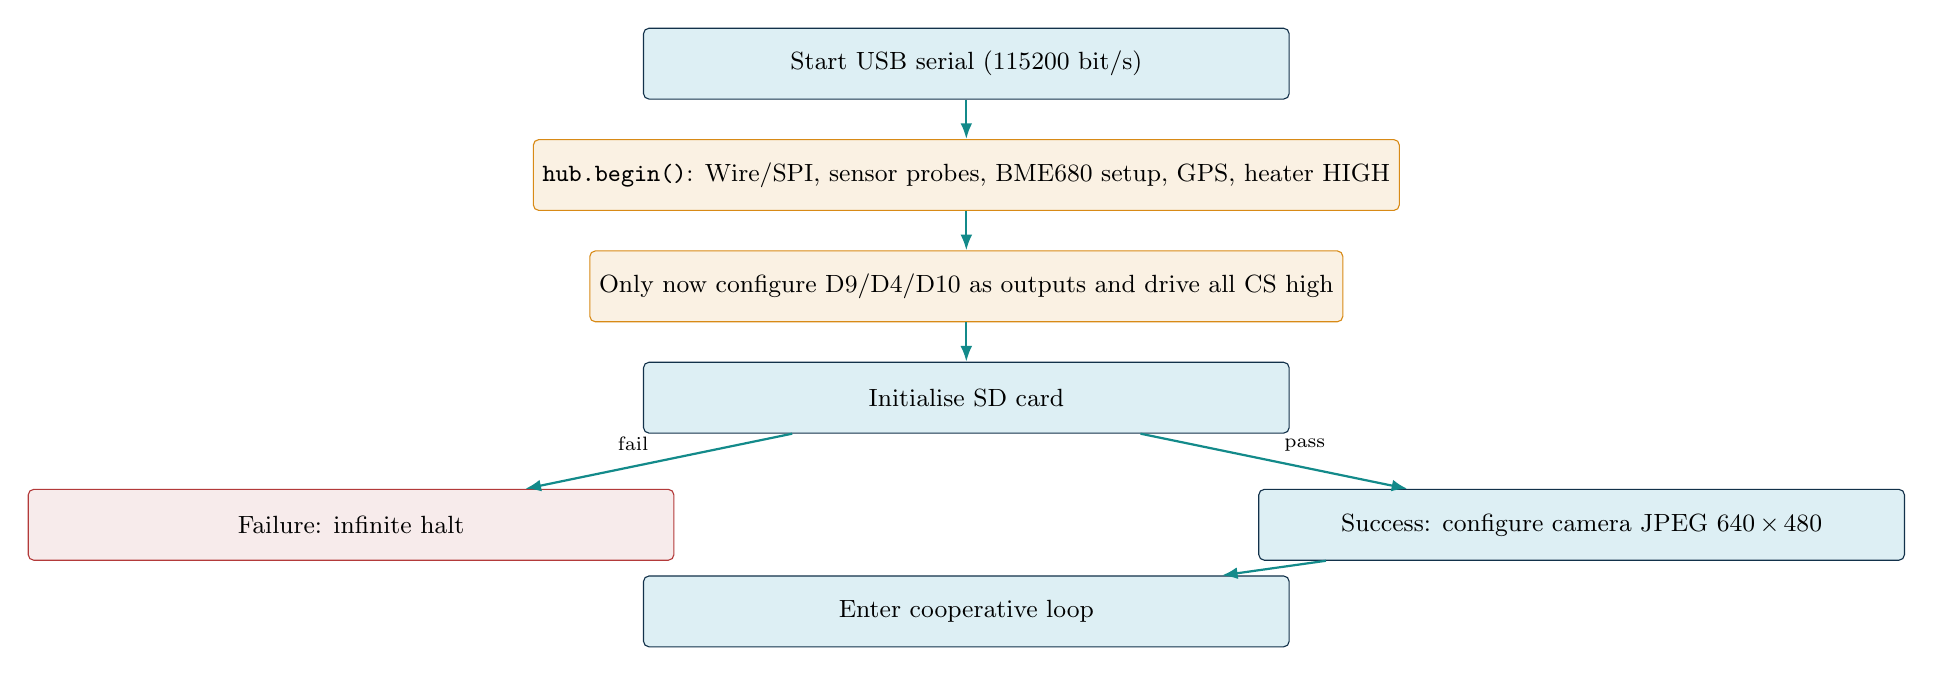
\begin{tikzpicture}[
  node distance=5mm,
  phase/.style={draw=navy,rounded corners=2pt,fill=sky,minimum width=82mm,
               minimum height=9mm,align=center,font=\small},
  warn/.style={draw=amber,rounded corners=2pt,fill=amber!12,minimum width=82mm,
               minimum height=9mm,align=center,font=\small},
  stop/.style={draw=redx,rounded corners=2pt,fill=redx!10,minimum width=82mm,
               minimum height=9mm,align=center,font=\small},
  arr/.style={-{Latex[length=2mm]},thick,draw=teal}
]
\node[phase] (serial) {Start USB serial (115200 bit/s)};
\node[warn,below=of serial] (hub) {\code{hub.begin()}: Wire/SPI, sensor probes, BME680 setup, GPS, heater HIGH};
\node[warn,below=of hub] (cs) {Only now configure D9/D4/D10 as outputs and drive all CS high};
\node[phase,below=of cs] (sd) {Initialise SD card};
\node[stop,below left=7mm and -4mm of sd] (halt) {Failure: infinite halt};
\node[phase,below right=7mm and -4mm of sd] (cam) {Success: configure camera JPEG 640\,$\times$\,480};
\node[phase,below=18mm of sd] (loop) {Enter cooperative loop};
\draw[arr] (serial)--(hub);
\draw[arr] (hub)--(cs);
\draw[arr] (cs)--(sd);
\draw[arr] (sd)--node[above left,font=\scriptsize]{fail}(halt);
\draw[arr] (sd)--node[above right,font=\scriptsize]{pass}(cam);
\draw[arr] (cam)--(loop);
\end{tikzpicture}
}
\caption{Implemented startup sequence. Amber blocks identify an ordering hazard: all shared-SPI chip selects should have deterministic inactive levels before any SPI peripheral is initialised. SD failure should enter a reported degraded state, not halt the entire acquisition system.}
\label{fig:startup}
\end{figure}

\subsection{Cooperative schedule}

The main loop polls USB input and drains GPS bytes as often as possible. Sensor updates are scheduled every 200 ms (nominally 5 Hz), text telemetry every 500 ms (2 Hz), and GPS summaries every 1000 ms (1 Hz). The subtraction form \code{now - last >= interval} is safe across \code{millis()} rollover. Nevertheless, this is a best-effort schedule, not a real-time guarantee: BME680 conversion, serial printing, image capture, and SD writes are blocking operations.

\begin{figure}[H]
\centering
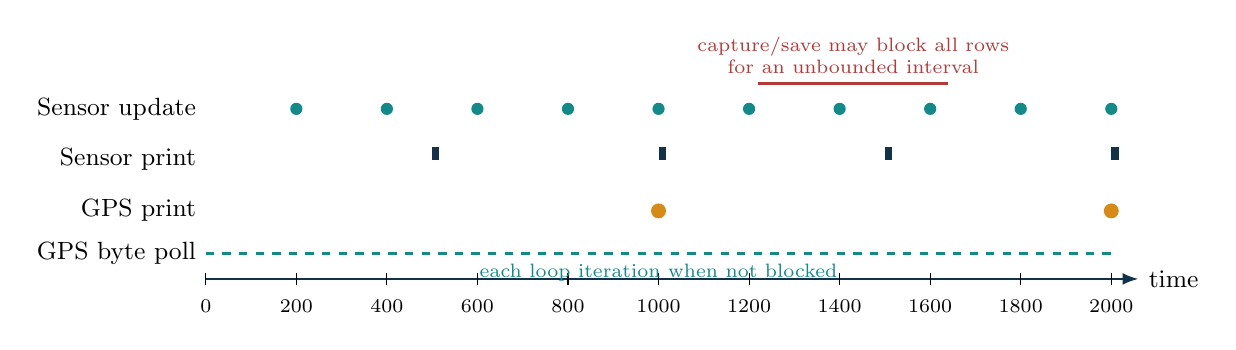
\begin{tikzpicture}[x=1.15cm,y=0.72cm,font=\small]
\draw[-{Latex[length=2mm]},thick,draw=navy] (0,0)--(10.3,0) node[right]{time};
\foreach \x/\lab in {0/0,1/200,2/400,3/600,4/800,5/1000,6/1200,7/1400,8/1600,9/1800,10/2000}
  {\draw (\x,0.1)--(\x,-0.1) node[below=2pt,font=\scriptsize]{\lab};}
\node[left] at (0,3.0) {Sensor update};
\node[left] at (0,2.1) {Sensor print};
\node[left] at (0,1.2) {GPS print};
\node[left] at (0,0.45) {GPS byte poll};
\foreach \x in {1,...,10}{\fill[teal] (\x,3.0) circle (2.2pt);}
\foreach \x in {2.5,5,7.5,10}{\fill[navy] (\x,2.1) rectangle +(0.08,0.22);}
\foreach \x in {5,10}{\fill[amber] (\x,1.2) circle (2.7pt);}
\draw[teal,thick,dashed] (0,0.45)--(10,0.45) node[midway,below,font=\scriptsize]{each loop iteration when not blocked};
\draw[redx,very thick] (6.1,3.45)--(8.2,3.45);
\node[redx,above,align=center,font=\scriptsize] at (7.15,3.45) {capture/save may block all rows\\for an unbounded interval};
\end{tikzpicture}
\caption{Nominal two-second execution timeline derived from the interval constants. Camera capture is asynchronous only at the command level; once started, completion polling and SD transfer are blocking.}
\label{fig:timing}
\end{figure}

\subsection{Image acquisition and shared-SPI arbitration}

Receiving \code{c} or \code{C} on USB serial triggers one frame. The camera FIFO is flushed, capture starts, and the firmware busy-waits for \code{CAP\_DONE\_MASK}. It accepts FIFO lengths from 1 byte through 2 MiB, creates \code{/IMG\%03d.JPG}, and transfers data through a 256-byte SRAM buffer. Each iteration reads one chunk from the camera using SPI mode 0 at 4 MHz, ends that transaction, selects SD, writes the chunk, and then re-enters camera burst mode. Figure~\ref{fig:spi} shows this deliberate bus hand-off.

\begin{figure}[H]
\centering
\resizebox{0.94\textwidth}{!}{%
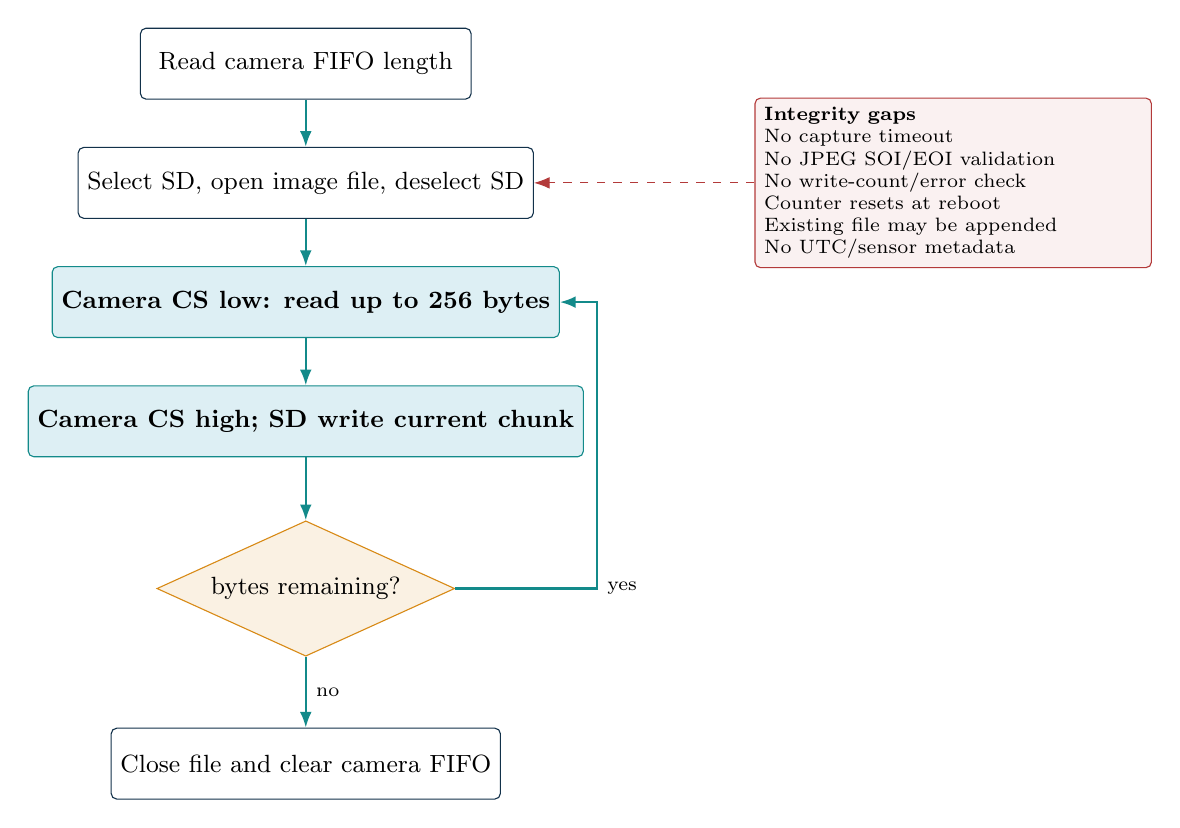
\begin{tikzpicture}[
  node distance=6mm,
  p/.style={draw=navy,rounded corners=2pt,fill=white,minimum width=42mm,
            minimum height=9mm,align=center,font=\small},
  active/.style={draw=teal,rounded corners=2pt,fill=sky,minimum width=42mm,
            minimum height=9mm,align=center,font=\small\bfseries},
  check/.style={diamond,draw=amber,fill=amber!12,aspect=2.2,align=center,font=\small},
  arr/.style={-{Latex[length=2mm]},thick,draw=teal}
]
\node[p] (len) {Read camera FIFO length};
\node[p,below=of len] (open) {Select SD, open image file, deselect SD};
\node[active,below=of open] (cam) {Camera CS low: read up to 256 bytes};
\node[active,below=of cam] (sd) {Camera CS high; SD write current chunk};
\node[check,below=8mm of sd] (more) {bytes remaining?};
\node[p,below=9mm of more] (done) {Close file and clear camera FIFO};
\draw[arr] (len)--(open);
\draw[arr] (open)--(cam);
\draw[arr] (cam)--(sd);
\draw[arr] (sd)--(more);
\draw[arr] (more.east)--++(18mm,0) node[right,font=\scriptsize]{yes} |- (cam.east);
\draw[arr] (more)--node[right,font=\scriptsize]{no}(done);
\node[draw=redx,fill=redx!7,rounded corners=2pt,align=left,font=\scriptsize,
      right=28mm of open,text width=48mm] (risks) {\textbf{Integrity gaps}\\No capture timeout\\No JPEG SOI/EOI validation\\No write-count/error check\\Counter resets at reboot\\Existing file may be appended\\No UTC/sensor metadata};
\draw[-{Latex[length=2mm]},draw=redx,dashed] (risks.west)--(open.east);
\end{tikzpicture}
}
\caption{Implemented camera-to-SD transfer and its integrity gaps. Chunking is memory-efficient, but a reliable data product also requires bounded capture, collision-free naming, marker or checksum validation, checked writes, and metadata linkage.}
\label{fig:spi}
\end{figure}

\subsection{GPS path}

\code{pollGPS()} continuously feeds available \code{Serial1} bytes to TinyGPSPlus. A position is considered current if the library marks it valid and its age is below two seconds. Latitude and longitude are updated only for such a fix; altitude and speed are updated whenever their individual fields are valid. The one-second console report includes position, altitude, speed, satellites, HDOP, and UTC time.

This is a reasonable non-blocking parser pattern for bench use. The startup ``found'' test, however, checks \code{Serial1.available()} once after a fixed 500-ms delay; absence of a byte at that instant is not a hardware diagnostic. More importantly, the NEO-6 data sheet specifies operational limits of 50 km altitude and 500 m/s for an airborne platform. A typical low-Earth-orbit CubeSat exceeds both. The receiver must therefore be treated as a ground-test aid, not an orbital-navigation subsystem.

\section{Data products and measurement semantics}

The GPS parsing pattern follows the TinyGPSPlus interface \cite{tinygps}; the orbital-use warning follows the receiver manufacturer's altitude and velocity limits \cite{neo6}.

\subsection{Present outputs}

Table~\ref{tab:data} distinguishes engineering units supplied by mature libraries from values that remain raw or ambiguous. This distinction should be retained in every future packet schema and user interface.

\begin{table}[H]
\centering
\caption{Current software outputs and measurement validity.}
\label{tab:data}
\begin{tabularx}{\textwidth}{P{0.20\textwidth}P{0.21\textwidth}P{0.17\textwidth}Y}
\toprule
Variable group & Source & Reported unit & Interpretation\\
\midrule
\code{accX/Y/Z} & ADXL345 Unified Sensor event & m/s\textsuperscript{2} & Engineering-unit output, but uncalibrated and not transformed to a spacecraft body frame.\\
\code{magX/Y/Z} & HMC5883 Unified Sensor event & $\mu$T & Engineering-unit output; magnetic bias/scale and on-board interference are not compensated.\\
\code{bmpTemp}, \code{bmpPressure} & BMP180 library & $^\circ$C, Pa & Library-compensated values; sampling mode and reference validation unrecorded.\\
\code{temperature}, \code{humidity}, \code{pressure} & BME680 library & $^\circ$C, \%, hPa & Explicit conversion of pressure from Pa to hPa; heater self-heating and enclosure effects remain.\\
\code{gasKOhm} & BME680 gas resistance & k$\Omega$ & Sensor resistance only; not a selective gas concentration or validated air-quality index.\\
\code{gyroX/Y/Z} & Direct L3G4200D registers & none / raw & Not valid as angular rate: device activation, signed 16-bit conversion, sensitivity scale, and bias calibration are missing.\\
\code{uvValue} & ADC A2 & count (0--1023) & Raw count; no reference-voltage measurement or UV transfer function.\\
\code{redValue}, \code{noxValue} & ADC A0/A1 & count (0--1023) & Raw count. Computed voltages assume exactly 5.000 V and are not printed. No ppm/ppb model.\\
GPS fields & TinyGPSPlus & degrees, m, km/h, satellites, HDOP & Parsed navigation metadata for terrestrial testing; receiver limits preclude normal LEO navigation.\\
Image & OV2640 FIFO to SD & JPEG, 640\,$\times$\,480 & File lacks capture UTC, sensor snapshot, sequence persistence, and integrity record.\\
\bottomrule
\end{tabularx}
\end{table}

\subsection{Recommended telemetry contract}

Human-readable serial prints are helpful during integration but unsuitable as the only data contract. A compact record should include a version, monotonic sequence, GPS UTC where available, controller time, sensor-health bitmap, calibrated values with fixed units, and a CRC. A corresponding image manifest should reference the same sequence and timestamp.

\begin{table}[H]
\centering
\caption{Minimum record schema for traceable sensing and imaging.}
\label{tab:schema}
\small
\begin{tabularx}{\textwidth}{P{0.25\textwidth}P{0.20\textwidth}Y}
\toprule
Field group & Example representation & Purpose\\
\midrule
Protocol identity & magic, version, length & Enables deterministic parsing and future schema evolution.\\
Time and order & boot ID, sequence, \code{millis}, UTC, UTC-valid flag & Distinguishes resets, stale fixes, dropped packets, and capture alignment.\\
Health & online, stale, saturated, and error bitmaps & Prevents plausible-looking default or stale values from being treated as observations.\\
Measurements & typed fixed- or floating-point fields plus unit definition & Eliminates ambiguity between raw counts, physical units, and calibrated products.\\
Image link & persistent image ID, byte count, CRC-32, capture status & Binds a JPEG to its contemporaneous state and verifies transfer integrity.\\
Packet integrity & CRC-16/CRC-32 & Detects corruption in storage and transport.\\
\bottomrule
\end{tabularx}
\end{table}

\section{Engineering findings and failure analysis}
\label{sec:findings}

Severity reflects potential impact on data correctness, system availability, or hardware safety. It does not estimate occurrence probability because no runtime or environmental test data are available.

\begin{longtable}{P{0.07\textwidth}P{0.10\textwidth}P{0.21\textwidth}P{0.24\textwidth}P{0.25\textwidth}}
\caption{Traceable engineering findings at commit \code{28d356c}.}\label{tab:findings}\\
\toprule
ID & Severity & Evidence & Consequence & Required correction\\
\midrule
\endfirsthead
\toprule
ID & Severity & Evidence & Consequence & Required correction\\
\midrule
\endhead
F-01 & \critical & Gyroscope boot code only checks ACK at \code{0x69}; no control-register write enables normal measurement. & Output registers may remain stale/power-down; a detected device is reported as operational. & Read WHO\_AM\_I, configure CTRL\_REG1/4, wait for startup, verify read-back and data-ready behaviour.\\
F-02 & \high & Two bytes are ORed directly into a float; no \code{int16\_t} cast, sensitivity, or bias correction. & Negative two's-complement rates can appear as large positive numbers; output has no defensible unit. & Assemble into \code{int16\_t}, apply the configured mdps/digit scale, subtract calibrated bias, and attach unit/status.\\
F-03 & \high & \code{while (!CAP\_DONE)} has no deadline or watchdog service. & Camera or bus fault can freeze GPS parsing, sensing, telemetry, and command handling indefinitely. & Add a bounded timeout, FIFO reset, retry budget, fault code, and transition to degraded operation.\\
F-04 & \high & \code{imgCount} starts at zero every boot and \code{FILE\_WRITE} appends to an existing file. & Reset followed by capture can concatenate JPEG streams and silently corrupt the image product. & Scan/restore a persistent sequence, reject existing names or open with create/truncate semantics, then verify close and byte count.\\
F-05 & \high & Shared-SPI CS pins become outputs/high only after \code{hub.begin()} performs BME680 SPI initialisation. & Floating CS inputs can select multiple peripherals during boot and cause contention or failed configuration. & Configure all CS pins and hardware SS as outputs/high before \code{SPI.begin()} or any peripheral begin call.\\
F-06 & \high & Probe results are printed but not retained; \code{update()} calls every sensor reader regardless of initialisation success. Several public fields are not initialised. & Missing-device failures may produce stale, undefined, or misleading values without machine-readable status. & Store per-device states, initialise all outputs to NaN/sentinel, gate reads, count errors, and report freshness.\\
F-07 & \high & SD failure enters an infinite loop. & Failure of optional storage disables navigation and all sensing, eliminating graceful degradation. & Use a system state machine; continue acquisition/telemetry without storage and allow bounded reinitialisation.\\
F-08 & \high & No schematic, power tree, regulator, level translator, BOM, or PCB files are versioned. & Voltage compatibility, heater drive, MISO contention, grounding, decoupling, and connector safety cannot be established. & Version the complete ECAD source and released manufacturing package; perform design-rule and electrical-rule review.\\
F-09 & \high & No watchdog, brownout recovery policy, reset-cause log, or persistent boot counter. & Transient faults can produce indefinite loss of function or untraceable resets. & Enable watchdog with scheduled service, record reset cause/boot ID, and implement bounded recovery paths.\\
F-10 & \high & NEO-6 operational limits are 50 km and 500 m/s; ordinary LEO exceeds both. & Receiver cannot be relied on for orbital position/velocity. & Select a space-appropriate GNSS receiver and validate its firmware mode, antenna, RF path, and mission orbit. Retain NEO-6M only for ground tests.\\
F-11 & \medium & Camera initialisation has no SPI test-register or sensor-ID check; ``ready'' is unconditional. & Cabling or sensor failure is discovered only indirectly, potentially after a blocking capture request. & Perform controller-register loopback, sensor-ID read, bounded self-test capture, and health-state update.\\
F-12 & \medium & FIFO validity uses length only; write return values and JPEG SOI/EOI markers are unchecked. & Truncated or non-JPEG data can be accepted as a successful capture. & Validate markers/length, check every write count, compute checksum, and record the result in a manifest.\\
F-13 & \medium & Analogue conversion assumes an exact 5-V reference; UV and gas channels lack calibration/warm-up models. & Raw counts cannot support quantitative environmental claims and will drift with supply/reference and temperature. & Measure/reference Vcc, characterise front ends, encode calibration coefficients, warm-up state, range, saturation, and uncertainty.\\
F-14 & \medium & README assigns camera CS D10 although code uses D9; GPS pins are labelled RX2/TX2 although code uses UART1. & Assembly from README can create a CS collision or UART wiring confusion. & Generate pin documentation from a single configuration source and correct the wiring table.\\
F-15 & \medium & Dependencies and board/compiler versions are absent; no automated build exists. & Future contributors cannot reproduce the same binary or distinguish source and toolchain regressions. & Add \code{arduino-cli.yaml}, pinned library index/versions, FQBN, build script, CI compile, and release hashes.\\
F-16 & \medium & Sensor values are printed but not stored; images have no timestamp or sensor snapshot. & Scientific traceability and cross-modal analysis are impossible after the live console session. & Log timestamped telemetry and an image manifest using a shared persistent sequence and integrity checks.\\
F-17 & \medium & Repository text contains character-encoding corruption and has no licence or contribution/test guidance. & Diagnostic output is difficult to interpret; reuse and maintenance conditions are ambiguous. & Normalise UTF-8 or ASCII diagnostics and add licence, architecture, build, wiring, calibration, and test documentation.\\
\bottomrule
\end{longtable}

\subsection{Root-cause relationships}

Most findings are not independent. The absence of a single configuration manifest produces the CS and UART documentation drift. The absence of an explicit system state model produces the fatal SD dependency, unconditional sensor reads, and unbounded camera wait. The absence of a data contract produces unit ambiguity, no health/freshness fields, and no image-to-telemetry linkage. Correcting those three architectural causes will remove more risk than isolated print-message edits.

\begin{figure}[H]
\centering
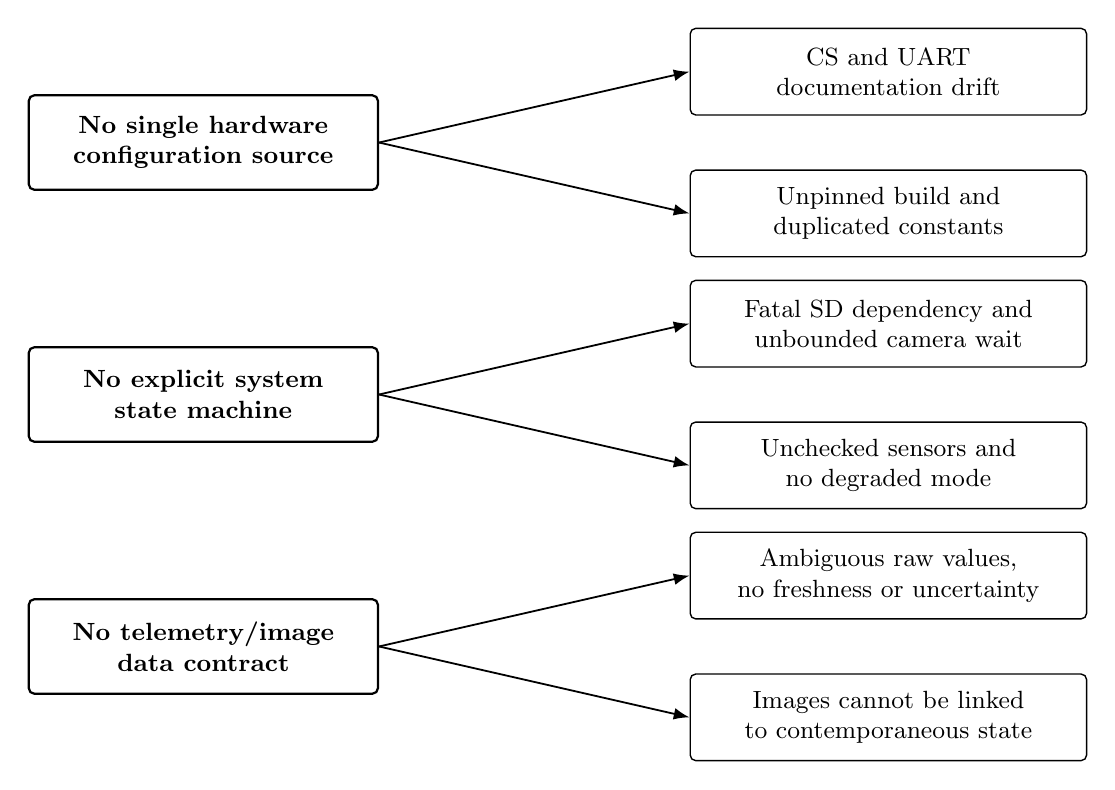
\begin{tikzpicture}[x=1cm,y=1cm,
  cause/.style={draw=black,line width=0.8pt,fill=white,rounded corners=2pt,
                text width=42mm,minimum height=12mm,align=center,font=\small\bfseries},
  effect/.style={draw=black,line width=0.5pt,fill=white,rounded corners=2pt,
                 text width=48mm,minimum height=11mm,align=center,font=\small},
  arr/.style={-{Latex[length=2mm]},line width=0.65pt,draw=black}
]
\node[cause] (cfg) at (0,4.6) {No single hardware\\configuration source};
\node[effect] (cs) at (8.7,5.5) {CS and UART\\documentation drift};
\node[effect] (build) at (8.7,3.7) {Unpinned build and\\duplicated constants};

\node[cause] (state) at (0,1.4) {No explicit system\\state machine};
\node[effect] (halt) at (8.7,2.3) {Fatal SD dependency and\\unbounded camera wait};
\node[effect] (health) at (8.7,0.5) {Unchecked sensors and\\no degraded mode};

\node[cause] (contract) at (0,-1.8) {No telemetry/image\\data contract};
\node[effect] (units) at (8.7,-0.9) {Ambiguous raw values,\\no freshness or uncertainty};
\node[effect] (trace) at (8.7,-2.7) {Images cannot be linked\\to contemporaneous state};

\draw[arr] (cfg.east)--(cs.west);
\draw[arr] (cfg.east)--(build.west);
\draw[arr] (state.east)--(halt.west);
\draw[arr] (state.east)--(health.west);
\draw[arr] (contract.east)--(units.west);
\draw[arr] (contract.east)--(trace.west);
\end{tikzpicture}
\caption{Architectural root causes and their downstream effects. The recommended roadmap targets configuration authority, state management, and data semantics before feature expansion.}
\label{fig:rootcause}
\end{figure}

\section{Recommended target architecture}

\subsection{Firmware state model}

The revised application should separate boot, acquisition, storage, and recovery concerns. Each peripheral should expose \code{init()}, \code{sample()}, \code{health()}, and bounded \code{recover()} operations. A top-level state machine should continue useful work when a non-essential device fails.

\begin{figure}[H]
\centering
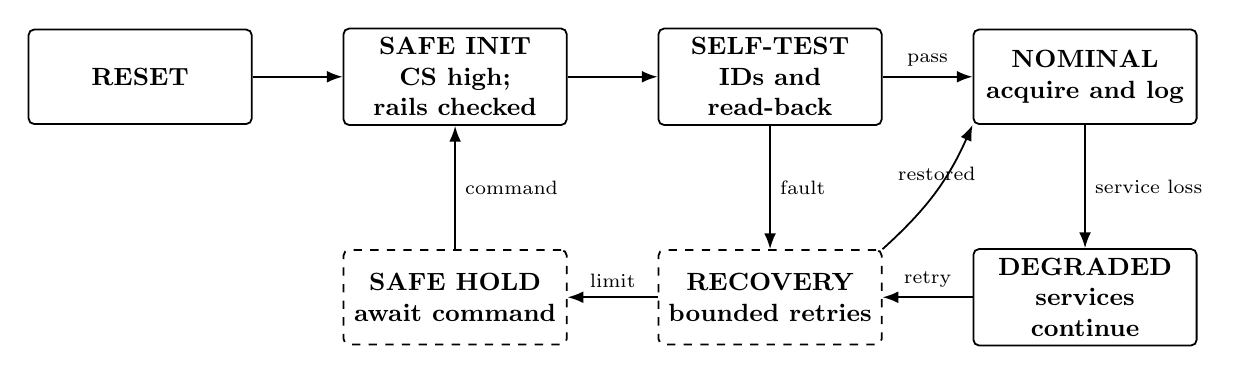
\begin{tikzpicture}[x=1cm,y=1cm,
  state/.style={draw=black,line width=0.65pt,rounded corners=2pt,fill=white,
                text width=26mm,minimum height=12mm,align=center,font=\small\bfseries},
  recovery/.style={draw=black,dashed,line width=0.65pt,rounded corners=2pt,fill=white,
                   text width=26mm,minimum height=12mm,align=center,font=\small\bfseries},
  arr/.style={-{Latex[length=2mm]},line width=0.65pt,draw=black}
]
\node[state] (reset) at (0,2.8) {RESET};
\node[state] (safe) at (4,2.8) {SAFE INIT\\CS high; rails checked};
\node[state] (self) at (8,2.8) {SELF-TEST\\IDs and read-back};
\node[state] (run) at (12,2.8) {NOMINAL\\acquire and log};
\node[state] (degraded) at (12,0) {DEGRADED\\services continue};
\node[recovery] (recover) at (8,0) {RECOVERY\\bounded retries};
\node[recovery] (safehold) at (4,0) {SAFE HOLD\\await command};

\draw[arr] (reset.east)--(safe.west);
\draw[arr] (safe.east)--(self.west);
\draw[arr] (self.east)--node[above,font=\scriptsize]{pass}(run.west);
\draw[arr] (self.south)--node[right,font=\scriptsize]{fault}(recover.north);
\draw[arr] (run.south)--node[right,font=\scriptsize]{service loss}(degraded.north);
\draw[arr] (degraded.west)--node[above,font=\scriptsize]{retry}(recover.east);
\draw[arr] (recover.north east) to[bend right=12]
  node[pos=0.52,above,font=\scriptsize]{restored} (run.south west);
\draw[arr] (recover.west)--node[above,font=\scriptsize]{limit}(safehold.east);
\draw[arr] (safehold.north)--node[right,font=\scriptsize]{command}(safe.south);
\end{tikzpicture}
\caption{Recommended bounded state machine. Optional storage or camera failure no longer suppresses sensing and fault telemetry; recovery attempts are finite and observable.}
\label{fig:statemachine}
\end{figure}

\subsection{Shared-bus ownership}

Create one SPI arbiter that owns D9, D10, and D4, configures deterministic inactive levels before starting SPI, and wraps every transaction in an interface that records device, mode, clock, timeout, and outcome. Device drivers should not independently hide chip-select pin numbers. An equivalent I\textsuperscript{2}C layer should bound requests, validate byte count, recover a stuck bus where electrically possible, and distinguish address ACK from identity/readiness.

\subsection{Measurement quality}

Every channel requires a documented transformation from raw data to a stated unit. At minimum, the inertial sensors need axis orientation, bias, scale, temperature dependence, saturation limits, and a calibration date/version. The magnetometer additionally requires hard-iron and soft-iron compensation in the integrated assembly. Analogue UV and gas channels need reference-voltage measurement, front-end transfer functions, warm-up state, environmental compensation, and uncertainty. Values that have not passed these steps should be labelled \emph{raw engineering telemetry}, not physical concentration or irradiance.

\subsection{Imaging integrity}

Image capture should be a non-blocking service with a deadline. On success, the storage layer should allocate a persistent identifier, create a new file without appending, validate JPEG boundaries, check each write count, close/synchronise, and calculate a checksum. The image manifest should carry capture start/end times, FIFO length, stored length, resolution, camera status, checksum, and the nearest telemetry sequence.

\section{Verification and validation plan}

The staged approach is consistent with NASA small-spacecraft development and test guidance \cite{nasa}.

The verification programme should advance only when the previous stage has objective evidence. Consumer-module operation on a desk is not a substitute for integrated CubeSat qualification, but it is the necessary first stage.

\begin{longtable}{P{0.10\textwidth}P{0.18\textwidth}P{0.30\textwidth}P{0.31\textwidth}}
\caption{Staged verification matrix and minimum acceptance evidence.}\label{tab:verification}\\
\toprule
Stage & Objective & Required activity & Minimum acceptance evidence\\
\midrule
\endfirsthead
\toprule
Stage & Objective & Required activity & Minimum acceptance evidence\\
\midrule
\endhead
V0 & Reproducible build & Pin board FQBN, Arduino core, all libraries, compiler, and build command; compile in CI with warnings enabled. & Clean build log, binary size report, dependency manifest, source commit, and binary checksum.\\
V1 & Static correctness & Unit-test signed gyro conversion, timeout arithmetic, filename allocation, packet encode/decode, CRC, and error transitions on a host where possible. & Automated tests with normal, boundary, wraparound, truncated, and fault cases.\\
V2 & Electrical bring-up & Verify every rail, reset level, CS default, I\textsuperscript{2}C pull-up, SPI MISO release, UART levels, ADC range, heater current, and peak/average current. & Annotated schematic, oscilloscope/logic-analyser captures, power table, and no absolute-maximum violations.\\
V3 & Per-device functional test & Read immutable IDs, configuration read-back, data-ready cadence, range/saturation, self-test where available, SD read/write, camera marker integrity, and GNSS stream. & Serial-numbered test report with pass/fail criteria and raw logs.\\
V4 & Integrated endurance & Run acquisition, GPS parsing, repeated images, and storage concurrently across multiple resets and full/removed/corrupt SD scenarios. Inject bus/device faults. & At least 24--72 h trace with zero unbounded hangs, quantified drop/error rates, reset-cause history, and recoverable files.\\
V5 & Calibration & Calibrate inertial, magnetic, pressure, temperature/humidity, UV, and gas paths against traceable references over expected range. & Coefficients with version, residual/error plots, uncertainty budget, and acceptance bounds.\\
V6 & Environmental engineering & Define mission profile, then perform thermal cycling/vacuum as applicable, vibration, shock, EMC, and radiation/parts analysis on representative hardware. & Approved procedures, before/during/after functional data, anomaly disposition, and margin assessment.\\
V7 & Mission acceptance & Repeat acceptance tests on the flight unit; verify software image, configuration, mass/power/data budgets, interfaces, and operational procedures. & Signed configuration index, acceptance report, released binary/hash, and closed waivers.\\
\bottomrule
\end{longtable}

\section{Prioritised remediation roadmap}
\label{sec:roadmap}

\begin{table}[H]
\centering
\caption{Recommended work packages in dependency order.}
\label{tab:roadmap}
\small
\begin{tabularx}{\textwidth}{P{0.12\textwidth}P{0.20\textwidth}Y P{0.22\textwidth}}
\toprule
Priority & Work package & Scope & Exit criterion\\
\midrule
P0 & Evidence and safe power-up & Add ECAD/BOM; resolve voltage domains and heater driver; drive all CS high before SPI; document authoritative pin map. & Electrical review closed and logic-analyser traces show contention-free boot.\\
P0 & Deterministic sensor correctness & Initialise/identify gyro, implement signed conversion and scaling, retain health flags, initialise all values, gate failed readers. & Known static/rotational inputs produce signed, scaled data and failures appear as explicit status.\\
P0 & Bounded execution & Add camera deadline, watchdog, nonfatal SD path, reset-cause log, and finite retry budgets. & Fault injection cannot create an indefinite loop; system continues in a declared degraded state.\\
P1 & Reproducible software & Pin toolchain/libraries, add CI compile and warnings, normalise encoding, add licence and build/test documentation. & Fresh clone builds deterministically and produces recorded binary/hash.\\
P1 & Traceable data products & Define packet/schema, timestamped SD telemetry, image manifest, persistent IDs, checked writes, JPEG validation, and CRC. & Every image is uniquely named, integrity-checked, and linked to a valid telemetry sequence.\\
P1 & Calibration and timing & Characterise every channel, use measured reference voltage, define body axes, schedule via deadlines, quantify sample age and jitter. & Calibration/uncertainty file is versioned and timing tests meet stated requirements.\\
P2 & CubeSat redesign choices & Replace/justify orbital GNSS, assess processor/storage architecture, parts lifecycle, radiation, thermal, vacuum, EMC, and power modes. & Mission requirements map to selected parts with margins and qualification strategy.\\
P2 & Qualification evidence & Execute integrated endurance and environmental programme with anomaly tracking. & Verification matrix is complete or formally waived by responsible engineering authority.\\
\bottomrule
\end{tabularx}
\end{table}

\section{Conclusion}

The \repo\ codebase demonstrates a credible first integration of heterogeneous sensors, an SPI FIFO camera, SD storage, and GPS on a resource-constrained ATmega2560. The 256-byte image-transfer buffer and explicit shared-SPI deselection show awareness of the platform's memory and bus constraints. The current repository is nevertheless an integration prototype, not a verified CubeSat PCB or flight subsystem.

The immediate defects are specific and correctable: initialise and scale the gyroscope, make all device failures machine-readable, establish inactive SPI states before any bus transaction, bound camera operations, allocate reset-safe image identifiers, validate stored data, and preserve acquisition when SD is unavailable. In parallel, the project needs the missing engineering record---schematic, PCB, BOM, power/interface analysis, reproducible build, calibration, and test evidence. The NEO-6M should remain a terrestrial test instrument and be replaced for orbital navigation.

If the P0 and P1 work packages are completed with the stated evidence, the repository can become a robust engineering-model baseline. Flight suitability can only be considered after mission-specific component selection and V2--V7 verification; it cannot be inferred from successful desk operation or from the firmware alone.

\clearpage
\appendix
\section{Code traceability index}

\small
\begin{longtable}{P{0.28\textwidth}P{0.24\textwidth}P{0.38\textwidth}}
\caption{Key implementation claims and source locations.}\label{tab:trace}\\
\toprule
Claim & Source location & Evidence\\
\midrule
\endfirsthead
\toprule
Claim & Source location & Evidence\\
\midrule
\endhead
Three SPI chip selects & \src{main.ino}{11--17} & Camera D9, SD D4, and BME680 D10.\\
CS arbitration helpers & \src{main.ino}{24--38} & All devices deselected; SD helper explicitly excludes camera and BME680.\\
Sensor setup precedes CS output setup & \src{main.ino}{45--55} & \code{hub.begin()} is called before pin modes and \code{deselectAll()}.\\
SD failure is fatal & \src{main.ino}{57--67} & Failed \code{SD.begin()} enters an infinite loop.\\
VGA JPEG camera setup & \src{main.ino}{69--78} & JPEG mode, OV2640 initialisation, and 640\,$\times$\,480 selection.\\
Nominal update/print periods & \src{main.ino}{104--157} & 200-ms sensor update, 500-ms sensor print, and 1000-ms GPS print.\\
Unbounded capture wait & \src{main.ino}{160--175} & Busy-wait has no deadline or escape condition.\\
Reset-unsafe filename & \src{main.ino}{19, 189--195} & RAM counter starts at zero and file opens with \code{FILE\_WRITE}.\\
Chunked transfer & \src{main.ino}{203--229} & 256-byte camera read followed by SD write and bus reacquisition.\\
BME680 settings & \src{SensorHub.cpp}{55--68} & 8$\times$/2$\times$/4$\times$ oversampling, IIR 3, and 320$^\circ$C/150-ms heater.\\
Gyroscope only probed & \src{SensorHub.cpp}{70--77} & I\textsuperscript{2}C ACK test at \code{0x69}; no identity/configuration write.\\
Unconditional sensor readers & \src{SensorHub.cpp}{98--106} & Every reader is called without stored online state.\\
Gyroscope conversion gap & \src{SensorHub.cpp}{149--158} & Six unchecked bytes are assembled directly into floating-point variables.\\
ADC reference assumption & \src{SensorHub.cpp}{166--173} & Gas voltage uses fixed \code{5.0/1023.0}.\\
GPS freshness rule & \src{SensorHub.cpp}{176--198} & Valid location younger than two seconds defines \code{gpsFix}.\\
README camera conflict & \src{readme.md}{94--105} & Camera CS documented as D10, conflicting with implemented D9/BME D10.\\
README UART label conflict & \src{readme.md}{82--90} & Pins 19/18 are labelled RX2/TX2 despite notes and code indicating UART1.\\
\bottomrule
\end{longtable}

\section{Proposed definition of done for the next release}

A release should not be called an engineering baseline until all of the following are true:

\begin{enumerate}
  \item A fresh clone compiles in CI using pinned core and library versions, with no errors and no unexplained warnings.
  \item The authoritative pin map, schematic, PCB, BOM, and firmware constants agree and are reviewed together.
  \item Every sensor is identified by device ID where available, configured by explicit register/settings, and represented by health/freshness state.
  \item Gyroscope output is signed, scaled to angular rate, calibrated, and tested for positive and negative rotation.
  \item Camera, SD, I\textsuperscript{2}C, and GPS faults are bounded; no injected peripheral fault can create an infinite wait.
  \item Reset cannot overwrite or append to an existing image; every file has checked length, integrity metadata, and a linked telemetry record.
  \item The software records reset cause, boot ID, sequence, UTC validity, monotonic time, and CRC-protected telemetry.
  \item Voltage compatibility, heater drive, current peaks, bus waveforms, and inactive-CS behaviour are demonstrated on the actual board.
  \item The intended mission profile is documented and every component, including GNSS, is screened against it.
  \item Calibration, endurance, and environmental evidence is versioned with serial-number and software-revision traceability.
\end{enumerate}

\clearpage
\sloppy
\raggedright
\begin{thebibliography}{99}

\bibitem{repo}
M. S. I. Siyam, ``sensorTest: ATmega2560 PRO Sensor Hub,'' GitHub repository, audited at commit \code{28d356c}, 2026. [Online]. Available: \url{https://github.com/SISIYAM/sensorTest}

\bibitem{atmega}
Microchip Technology Inc., ``ATmega2560 8-bit AVR Microcontroller,'' product documentation. [Online]. Available: \url{https://www.microchip.com/en-us/product/atmega2560}

\bibitem{mega}
Arduino, ``Arduino Mega 2560 Rev3---Datasheet and Pinout,'' 2026. [Online]. Available: \url{https://docs.arduino.cc/resources/datasheets/A000067-datasheet.pdf}

\bibitem{sd}
Arduino, ``SD Library Documentation,'' version 1.3.0, 2026. [Online]. Available: \url{https://docs.arduino.cc/libraries/sd}

\bibitem{bme680}
Bosch Sensortec, ``BME680 Low-Power Gas, Pressure, Temperature and Humidity Sensor,'' product page and BST-BME680-DS001 data sheet. [Online]. Available: \url{https://www.bosch-sensortec.com/en/products/environmental-sensors/gas-sensors/bme680}

\bibitem{adxl}
Analog Devices, ``ADXL345: 3-Axis, $\pm$2 g/$\pm$4 g/$\pm$8 g/$\pm$16 g Digital Accelerometer,'' Data Sheet, Rev. G. [Online]. Available: \url{https://www.analog.com/media/en/technical-documentation/data-sheets/adxl345.pdf}

\bibitem{l3g}
STMicroelectronics, ``L3G4200DH MEMS Motion Sensor: Three-Axis Digital Output Gyroscope,'' Data Sheet, Doc. ID 17300 Rev. 1. [Online]. Available: \url{https://www.st.com/resource/en/datasheet/l3g4200dh.pdf}

\bibitem{neo6}
u-blox AG, ``NEO-6 u-blox 6 GPS Modules Data Sheet,'' GPS.G6-HW-09005-E. [Online]. Available: \url{https://content.u-blox.com/sites/default/files/products/documents/NEO-6_DataSheet_%28GPS.G6-HW-09005%29.pdf}

\bibitem{mics}
SGX Sensortech, ``MiCS-4514 Combined CO and NO\textsubscript{2} Sensor,'' product documentation. [Online]. Available: \url{https://sgxsensortech.com/sensor/mics-4514}

\bibitem{arducam}
Arducam, ``Legacy SPI Camera / OV2640 2MP Plus Documentation,'' product documentation. [Online]. Available: \url{https://docs.arducam.com/Arduino-SPI-camera/Legacy-SPI-camera/}

\bibitem{tinygps}
M. Hart, ``TinyGPSPlus: A Full-Featured GPS/NMEA Parser for Arduino,'' project repository. [Online]. Available: \url{https://github.com/mikalhart/TinyGPSPlus}

\bibitem{nasa}
NASA Small Spacecraft Systems Virtual Institute, ``Small Spacecraft Body of Knowledge and CubeSat 101 Resources,'' 2026. [Online]. Available: \url{https://www.nasa.gov/smallsat-institute/small-spacecraft-body-of-knowledge/}

\end{thebibliography}

\end{document}
